% Results. One subsection per question of Figure 2; each opens with its question and closes with its answer.
% Every number carries its claim-ledger id (docs/neuralese-paper-log.md section 2) in a comment at the end of its line.
\section{Results}\label{sec:results}

We take the four questions of \cref{fig:questions} in turn.
\Cref{sec:q1,sec:q2} use Exp~21, \cref{sec:q3} uses Exp~22, and \cref{sec:q4} uses Exp~23 and Exp~16.

%-------------------------------------------------------------------------------------------------
\subsection{Q1: Does a blend of two candidates survive the layers?}\label{sec:q1}

If \ST{} carried two candidates forward, a blend of them would have to survive the forward pass.
We measure this with the method of \citet{backour2026dynamics}.
At each fork we feed $\alpha\,e(A) + (1-\alpha)\,e(B)$ for $\alpha = 0, 0.1, \dots, 1$ from the same cached prefix, % SETUP
where $A$ is the chosen token and $B$ the runner-up.
At every layer we project the hidden state onto the line from the state for the pure runner-up to the state for the
pure chosen token, which gives a position $c(\alpha)$ between 0 and 1.
Snap is the mean of $|c(\alpha) - \alpha|$, divided by the same quantity for a perfect switch at $\alpha = 0.5$. % SETUP
A snap of 0 means the blend is carried linearly, and 1 means a clean switch to one candidate.
On our grid, snap is 1 minus the CALIB score of \citet{backour2026dynamics}.
At the input the position equals the mixing weight, as it must (largest error $1.5 \times 10^{-7}$). % C21.2

\begin{figure}[t]
\centering
\begin{minipage}[c]{3.2in}
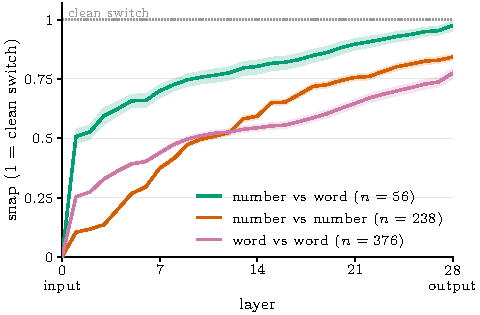
\includegraphics{fig3.pdf}
\end{minipage}\hfill
\begin{minipage}[c]{3.1in}
\caption{Blends collapse gradually through the layers.
At each fork we feed a blend of the chosen token and the runner-up and measure how sharply each layer
resolves it (snap: 0 = carried linearly, 1 = clean switch).
Snap is 0 at the input by construction and reaches 0.98 (number vs word), 0.84 (number vs number) % C21.4
and 0.77 (word vs word) at the output. % C21.4
Number vs word snaps hardest at every layer from 1 to 28; number vs number starts slowest % C21.24
and passes word vs word at layer 13. % C21.23
Bands: 95\% bootstrap CIs over problems.
670 unique forks from 40 GSM8K problems (items 10--49). % C21.1 C21.3
Inputs are sweeps between two candidates at forks, not the lopsided blends real runs feed (\cref{sec:q3}).}
\label{fig:snap}
\end{minipage}
\end{figure}

\Cref{fig:snap} shows the result for the 670 unique forks of Exp~21. % C21.1
Snap rises from 0 at the input to between 0.37 and 0.70 at layer 7, % C21.4
and to between 0.77 and 0.98 at the output. % C21.4
How far the two candidates differ in kind matters at the output.
Number vs word snaps hardest (0.98, 95\% CI [0.95, 1.00]), % C21.4 C21.5
then number vs number (0.84 [0.83, 0.86]) % C21.4 C21.5
and word vs word (0.77 [0.75, 0.79]). % C21.4 C21.5
This order holds at the output, not at every layer.
Number vs word is highest at every layer from 1 to 28, % C21.24
but number vs number starts slowest: it is below word vs word at layers 1 to 12 % C21.23
and above it from layer 13 to the output. % C21.23
At an exact 50/50 input, the next token is the pure chosen token's or the pure runner-up's % C21.6
at 95\% (number vs number), 98\% (number vs word) and 88\% (word vs word) of the forks where the two differ. % C21.6
The blended states also stay close to the line between the two pure states:
for number vs number at the output, the distance off the line is 0.28 of the distance between them. % C21.13
The noise that produced the trace does not change how a blend is processed
(number vs number at the output: 0.85 for forks from vanilla traces, 0.84 from Gumbel traces). % C21.14
Both pre-registered predictions on collapse were met (P1, P2; \cref{app:prereg}).

\paragraph{Answer.}
Only partly.
By the output a 50/50 blend is mostly resolved, and the next token follows one of the two candidates
at 88 to 98\% of forks. % C21.6
The collapse is gradual, though: at layer 7 the blend is still far from a clean switch. % C21.4
Whether the runner-up is lost or only absent from the next-token prediction is the next question.

%-------------------------------------------------------------------------------------------------
\subsection{Q2: Is the runner-up stored, and can later text read it back?}\label{sec:q2}

The next-token prediction is not the only place a candidate can survive.
Later steps attend to the keys and values (K,V) of the fork position, so the runner-up could be kept there.
We test this at the forks where the model followed the chosen token at the 50/50 input:
96 number vs number forks from 35 problems and 139 word vs word forks from 40 problems, % C21.28
plus 34 number vs word forks. % C21.7-8

\paragraph{Readback.}
For each fork we build two caches: one with the 50/50 blend of the chosen token and the runner-up at the fork
position, and a control cache with a 50/50 blend of the chosen token and a control token.
The control token is the third-ranked pre-noise candidate, so it also fits the context but holds no runner-up.
We then force a 64-token continuation into both caches. % C21.26
It is either the runner-up's own continuation, or the model's own continuation of the chosen token.
At each forced position we take the model's next-token distribution $p$ at the sampling temperature and place it
on the line from the distribution $p_B$ after the pure runner-up to the distribution $p_A$ after the pure chosen token:
$c = (p - p_B)\cdot(p_A - p_B) / \lVert p_A - p_B\rVert^2$. % SETUP
A score of 1 means ``as if the chosen token had been written'' and 0 ``as if the runner-up had been written''.
The runner-up readback is the control score minus the blend score.
It is above 0 when the blend cache makes the model read the text more as if it had written the runner-up.
Positions where $p_A$ and $p_B$ differ by less than 0.05 in total variation are skipped. % SETUP

\begin{figure}[t]
\centering
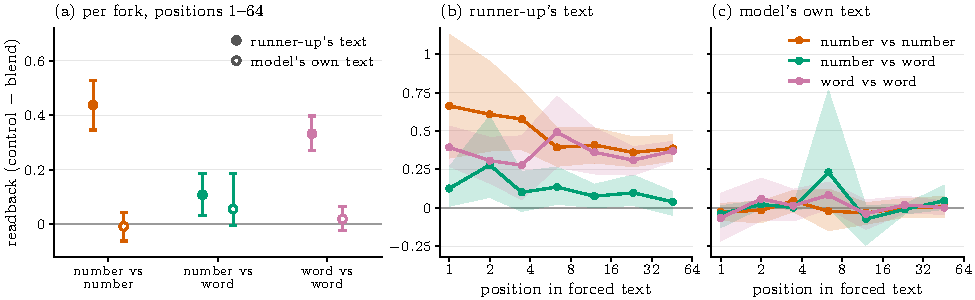
\includegraphics{fig4.pdf}
\caption{The runner-up is stored and can be read back, but stays dormant on the model's own path.
At forks where the model followed the chosen token, we force a 64-token continuation into the cache built from % C21.26
the 50/50 blend and into a control cache (chosen token blended 50/50 with the third-ranked candidate), and score the next-token
predictions from 0 (as if the runner-up had been written) to 1 (as if the chosen token had).
Readback = control minus blend; above 0 means the runner-up is read back from the cache.
(a) Per fork: with the runner-up's text, +0.44 (number vs number), +0.11 (number vs word) % C21.7-8
and +0.33 (word vs word); % C21.7-8
with the model's own text, $-0.01$ to $+0.06$, with every CI including 0. % C21.9 C21.25
(b) With the runner-up's text, the readback stays above 0 in every position bin up to 64 tokens % C21.26
for number vs number and word vs word.
(c) With the model's own text, the CI includes 0 in every bin for number vs number and word vs word. % C21.27
Positions are binned on a log scale; \cref{fig:readback-unbinned} shows them unbinned.
Bars and bands: 95\% bootstrap CIs over problems.
$n$ = 96, 34 and 139 forks. % C21.7-8
Exact 50/50 blends are the most favourable case for the runner-up, so these values are likely an upper bound for real forks,
if readback grows with the residual (\cref{sec:q3}).}
\label{fig:readback}
\end{figure}

With the runner-up's text, the blend cache reads it back (\cref{fig:readback}a).
The readback is $+0.44$ for number vs number (95\% CI [0.35, 0.53]), % C21.7-8
$+0.33$ for word vs word ([0.27, 0.40]) % C21.7-8
and $+0.11$ for number vs word ([0.03, 0.19]). % C21.7-8
The stored runner-up moves the model 0.44 of the way, % C21.7-8
on number vs number forks, toward reading the text as if it had written the runner-up itself.
For number vs word the runner-up is mostly erased, but not completely.
The effect lasts: for number vs number and word vs word the CI stays above 0 in every position bin up to 64 tokens % C21.26
(\cref{fig:readback}b), and without binning the mean is above 0 at every single position from 1 to 16 % C21.38
(\cref{fig:readback-unbinned}).
With the model's own text the picture is different (\cref{fig:readback}c).
The readback is $-0.01$ [$-0.06$, 0.04] for number vs number, % C21.9 C21.25
$+0.02$ [$-0.02$, 0.07] for word vs word % C21.9 C21.25
and $+0.06$ [$-0.00$, 0.19] for number vs word, % C21.9 C21.25
and the CI includes 0 in every position bin for number vs number and word vs word. % C21.27
On the path the model actually takes, the runner-up is dormant.
These results met pre-registered predictions P3 and P4 (\cref{app:prereg}).

\paragraph{Where the runner-up is stored.}
To locate it, we swap only the fork position's keys and values between the blend cache and the control cache,
at one layer or one block of layers, and force the runner-up's text as before.
\emph{Remove} puts the control's K,V into the blend cache and asks whether these layers are needed.
\emph{Insert} puts the blend's K,V into the control cache and asks whether they are enough.
We report the pooled share of the blend--control readback gap that the swap closes, summed over forks.

\begin{figure}[t]
\centering
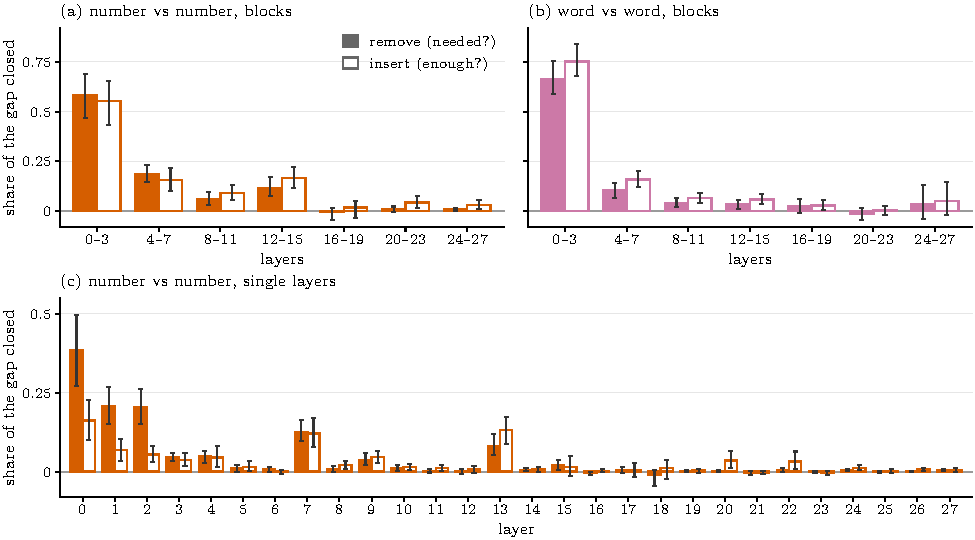
\includegraphics{fig5.pdf}
\caption{The runner-up is stored mostly in the early layers.
At each fork (50/50 blend; forks where the model followed the chosen token) we swap the keys and values of the
fork position between the blend cache and the control cache at a set of layers, and report the pooled share of
the blend--control readback gap this closes (summed over forks).
Remove (filled): put control K,V into the blend cache (are these layers needed?).
Insert (open): put blend K,V into the control cache (are they enough?).
(a, b) Layers 0--7 close 0.77 / 0.71 (number vs number, remove / insert) % C21.10
and 0.77 / 0.91 (word vs word) of the gap; % C21.10
layers 12--27 close 0.12 / 0.26 and 0.08 / 0.14. % C21.11
(c) Number vs number, single layers: the early effect sits in layers 0--2 % C21.19 C21.29
(remove 0.38, 0.21, 0.20). % C21.19 C21.29
Outside layers 0--3, only layers 7 (0.13 / 0.12) and 13 (0.08 / 0.13) stand out, with CIs excluding 0; % C21.19 C21.20 C21.30
every other layer closes at most 0.05. % C21.30
Note the different $y$-axis in (c).
The single-layer analysis was not pre-registered; \cref{tab:fig5-singles} shows these layers survive a
Bonferroni correction over all 56 single-layer tests. % C21.35
\Cref{tab:fig5-robust} shows the shares hold when any one problem, or forks with a small gap, are dropped;
\cref{fig:perfork} shows the per-fork spread, which is wide for layer 0.
Error bars: 95\% bootstrap CIs over problems.
96 forks from 35 problems (number vs number) and 139 forks from 40 problems (word vs word). % C21.28
Number vs word is not shown: its gap ($+0.11$) is too small to localise (\cref{tab:fig5-nw}). % C21.7-8
All shares are measured at exact 50/50 blends, the most favourable case for the runner-up, so these shares are likely an upper bound for real forks.}
\label{fig:patch}
\end{figure}

The runner-up is held mostly in layers 0 to 7 (\cref{fig:patch}a,b). % C21.10
These layers close a pooled share of 0.77 (remove) and 0.71 (insert) of the gap for number vs number, % C21.10
and 0.77 and 0.91 for word vs word. % C21.10
Layers 12 to 27 close 0.12 and 0.26, and 0.08 and 0.14. % C21.11
This split was pre-registered (P5, P6; the smallest lower bound of the difference is 0.31). % C21.22
By blocks of four layers, layers 0--3 carry most of it % C21.15 C21.17
(number vs number 0.58 / 0.55, word vs word 0.66 / 0.75 for remove / insert), % C21.15 C21.17
layers 4--7 add 0.19 / 0.16 and 0.10 / 0.16, % C21.15 C21.17
and every block from layer 16 on closes at most 0.04 for number vs number. % C21.16
For word vs word every block from layer 8 on closes at most 0.07. % C21.18
Across blocks the effects add up: the number vs number blocks sum to 0.95 (remove) and 1.06 (insert). % C21.21

Two findings below this level are exploratory: we found them after looking at the data.
First, for number vs number the early effect sits in layers 0 to 2 (\cref{fig:patch}c). % C21.29
Single layers close 0.38 / 0.16 (layer 0), 0.21 / 0.07 (layer 1) and 0.20 / 0.05 (layer 2). % C21.19 C21.29
Outside layers 0--3 only layers 7 (0.13 / 0.12) and 13 (0.08 / 0.13) stand out; % C21.19 C21.30
every other layer closes at most 0.05. % C21.30
All five survive a Bonferroni correction over the 56 single-layer tests, % C21.35
although the insert effects of layers 1 and 2 only just do (corrected lower bound 0.01; \cref{tab:fig5-singles}). % C21.35
Second, inside layers 0--3 single layers do not add up to their block. % C21.31
Removing one layer at a time sums to 0.84 against 0.58 for the block, % C21.31
and inserting one at a time sums to 0.32 against 0.55. % C21.31
One reading is that the runner-up is held redundantly across layers 0--2: % C21.29
removing any one of them breaks the readback, but no single one carries it.
Another is that the readback score saturates, since it is a projection that can pass 1.
Our data do not separate the two.

The pooled shares are not driven by one problem or a few forks.
Dropping any one problem changes a pooled share by at most 0.04, % C21.33
and keeping only forks with a gap of at least 0.1 changes none by more than 0.03 (\cref{tab:fig5-robust}). % C21.40
The 10 forks with the largest gap carry 0.27 (number vs number) and 0.24 (word vs word) of the total gap. % C21.37
Layer 0 is the exception to a uniform picture (\cref{fig:perfork}).
Its pooled remove share is 0.38, but the median fork's share is 0.12 % C21.34
(insert: 0.16 against 0.02), with quartiles of 0.01, 0.12 and 0.68. % C21.34 C21.39
Layer 0 matters a lot at some forks and little at about half of them.

Part of the early-layer share is expected by construction.
At layer 0 the keys and values of the fork position depend only on the fed embedding, which contains the runner-up,
so the runner-up is present there as an echo of the input.
There is also a small processed trace: for number vs number, layers 7 and 13 stand out (exploratory, as above). % C21.19

\paragraph{Answer.}
Yes.
The runner-up is stored, mostly in the keys and values of layers 0 to 7 and partly as an echo of the input, % C21.10
and text that turns toward it reads it back for the whole 64-token continuation. % C21.26
On the model's own path it stays dormant.
All of this is measured at exact 50/50 blends, the most favourable case for the runner-up.

%-------------------------------------------------------------------------------------------------
\subsection{Q3: What blends does the noise actually feed?}\label{sec:q3}

\Cref{sec:q1,sec:q2} feed exact 50/50 blends.
Real runs feed whatever blend the noise produces, so we record it.
Exp~22 replays ordinary vanilla, Gumbel and Dirichlet runs on 20 problems and logs the pre-noise and the fed weights % C22.7
at every thinking step.
Forks make up 9.2\% (vanilla), 13.0\% (Gumbel) and 13.3\% (Dirichlet) of thinking steps. % C22.1 C22.2 C22.3
There are 3,774, 5,761 and 4,978 forks; each arm is its own run, so the forks differ. % C22.7

\paragraph{The top token of \GST{} is a sampled token.}
Gumbel noise makes the top token of the fed blend a sample from the filtered distribution.
This is the Gumbel-max trick \citep{gumbel1954statistical,maddison2014sampling}:
the token with the largest perturbed log-probability is distributed exactly as a draw from the distribution, and the
softmax at temperature $\tau$ does not change which token is largest.
\citet{wu2025single} cite the trick to motivate Gumbel-Softmax; we check its consequence in the logged runs.
At forks, Gumbel makes a token other than the pre-noise top token the winner at a rate of 0.45, % C22.4
and ordinary sampling would do so at 0.45 (one minus the pre-noise top weight). % C22.4
The difference is 0.00 (95\% CI [$-0.01$, 0.02]). % C22.8
Binned by the sampling rate, Gumbel stays within 0.04 of sampling in every bin with at least 100 forks % C22.9
(\cref{fig:fed}b).
Dirichlet noise has no such guarantee, and it does not match sampling:
it flips less often, by $-0.03$ [$-0.04$, $-0.02$], and is below sampling in all 10 bins. % C22.8 C22.10
Its winner leans toward the pre-noise top token.
So Dirichlet \ST{} is not sampling in disguise in the exact sense that \GST{} is.

\begin{figure}[t]
\centering
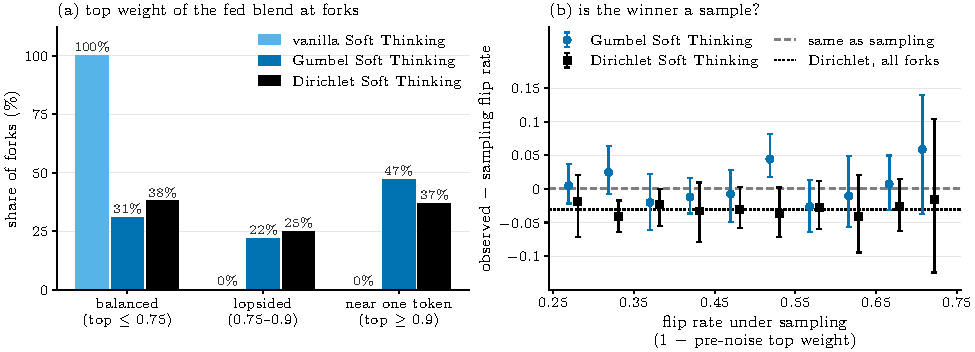
\includegraphics{fig6.pdf}
\caption{Noise turns real forks into lopsided blends, and Gumbel's winner is a sample.
A fork is a thinking step where the pre-noise runner-up holds at least 25\% of the weight % SETUP
(9.2\% of steps for vanilla, 13.0\% for Gumbel, 13.3\% for Dirichlet). % C22.1 C22.2 C22.3
(a) Share of forks by the top weight of the blend actually fed.
Vanilla feeds the pre-noise weights unchanged, so it shows what the model wanted: every fork is balanced % C22.5 C22.11
(top weight at most 0.75, by the fork rule). % C22.11
Gumbel feeds a near one-token blend (top weight at least 0.9) at 47\% of forks and Dirichlet at 37\%. % C22.11
The median fed blend has a residual (weight off the top token) of 0.12 for Gumbel and 0.17 for Dirichlet, % C22.12
against 0.44 before noise. % C22.12
(b) How often noise makes a token other than the pre-noise top one the winner, minus how often ordinary sampling
would (1 minus the pre-noise top weight), with forks binned by the sampling rate.
Gumbel matches sampling: 0.00 [$-0.01$, 0.02] overall and within 0.04 in every bin with at least 100 forks. % C22.8 C22.9
Dirichlet flips less often than sampling in every bin, $-0.03$ [$-0.04$, $-0.02$] overall (dashed line). % C22.8 C22.10
Vanilla never flips (not shown). % C22.1
Error bars: 95\% bootstrap CIs over problems.
3,774 (vanilla), 5,761 (Gumbel) and 4,978 (Dirichlet) forks from 20 GSM8K problems; % C22.7
each arm is its own run, so the forks differ.}
\label{fig:fed}
\end{figure}

\paragraph{The residual is real but small.}
Before noise, the median fork has a residual of 0.44: the model splits its weight. % C22.12
Vanilla feeds these weights unchanged, so every vanilla fork is balanced, % C22.5 C22.11
with a top weight of at most 0.75 by the fork rule (\cref{fig:fed}a). % C22.11
Noise makes the fed blends lopsided.
\GST{} feeds a blend near one token (top weight at least 0.9) at 47\% of forks, % C22.2 C22.11
a lopsided blend (0.75 to 0.9) at 22\% and a balanced one at 31\%. % C22.11
The median fed blend has a top weight of 0.88 and a residual of 0.12. % C22.2 C22.12
Dirichlet gives 37\%, 25\% and 38\%, with a median residual of 0.17. % C22.11 C22.12
At the median fork, almost all of the residual sits on one other token % C22.12
(0.99 of it for Gumbel and 1.00 for Dirichlet). % C22.12
Over all thinking steps, the fed blend is near one token at 85\% (Gumbel) % C22.2
and 83\% (Dirichlet) of steps. % C22.3
We had pre-registered that Gumbel would feed near one-token blends at 70\% or more of forks and 90\% or more % PR(Exp 22 P1, Exp 22 P3)
of steps; both failed (\cref{app:prereg}).

\paragraph{Answer.}
\GST{} feeds the sampled token plus a residual.
At forks the residual is real but small: its median is 0.12, % C22.12
and at about half of forks the blend is near one token. % C22.11
The exact 50/50 blends of \cref{sec:q1,sec:q2} are the extreme case, so the storage and readback measured there are
likely an upper bound on what a real fork carries, if readback grows with the residual.

%-------------------------------------------------------------------------------------------------
\subsection{Q4: Does the model use the residual?}\label{sec:q4}

If the top token of \GST{} is a sampled token, any difference from sampling must come from the residual.
Exp~23 isolates it.
Three arms run in lockstep on 100 GSM8K problems never used before (items 50--149), % C23.1
with shared Gumbel noise keyed by seed, step and token id.
\emph{Sampling} feeds the top token alone (a one-hot input).
\emph{\ST{}} feeds the full Gumbel blend.
The \emph{\ctrl{}} keeps the top token at its blend weight and moves the residual onto a random vocabulary token.
Because the noise is shared, the three arms pick the same top token at a step until their contexts differ,
and they differ only in where the residual goes.
The random rows have the same median norm as all real-token rows, and 0.994 of that of reasoning tokens (\cref{app:norms}), % C23.10 C23.11
so the control carries a residual of the same size and a typical norm.

\begin{table*}[t]
\centering
\small
\caption{Neither Gumbel Soft Thinking nor the random-residual control differs detectably from sampling in accuracy, and the paired intervals still allow differences of several points either way. Accuracy comparison: sampling and Gumbel Soft Thinking at seeds 0 and 1 on the same 30 problems, so their 60 runs are clustered by problem and their CIs are 95\% bootstrap intervals over problems (per seed: sampling 27 and 25 of 30, Gumbel 26 and 26); vanilla Soft Thinking has one seed and a Wilson interval. Its difference from sampling is paired on seed 0 (Newcombe interval); Gumbel's is the mean per-problem difference over both seeds, bootstrapped over problems. McNemar uses the seed 0 runs, the only seed vanilla has. Vanilla hit Cold Stop on 14 of 30 runs, and all 5 runs without an answer ended there; against Gumbel (seed 0) it is 1 vs 5, $p = 0.22$. Coupled ablation: seed 0; the three arms share their noise, and the random-residual control moves the residual to a random token. Accuracy has Wilson intervals and the paired difference a Newcombe hybrid-score interval. Its problems are not used in any other experiment. McNemar: exact two-sided test on the problems where exactly one of the pair is correct.}
\label{tab:accuracy}
\begin{tabular}{@{}lrrccccc@{}}
\toprule
 & & & & & \multicolumn{3}{c}{McNemar vs sampling} \\
\cmidrule(lr){6-8}
Arm & Runs & Correct & Accuracy [95\% CI] & Difference vs sampling [95\% CI] & Arm only & Sampling only & $p$ \\
\midrule
\multicolumn{8}{@{}l}{\emph{Accuracy comparison: GSM8K items 0--29}} \\
Sampling & 60 & 52 & 0.87 [0.75, 0.97] &  &  &  &  \\
Vanilla Soft Thinking & 30 & 22 & 0.73 [0.56, 0.86] & $-$0.17 [$-$0.33, $-$0.01] & 0 & 5 & 0.06 \\
Gumbel Soft Thinking & 60 & 52 & 0.87 [0.73, 0.97] & 0.00 [$-$0.10, +0.10] & 1 & 2 & 1.00 \\
\addlinespace
\multicolumn{8}{@{}l}{\emph{Coupled ablation: GSM8K items 50--149, arms in lockstep}} \\
Sampling & 100 & 86 & 0.86 [0.78, 0.91] &  &  &  &  \\
Gumbel Soft Thinking & 100 & 88 & 0.88 [0.80, 0.93] & +0.02 [$-$0.05, +0.09] & 6 & 4 & 0.75 \\
Random-residual control & 100 & 82 & 0.82 [0.73, 0.88] & $-$0.04 [$-$0.11, +0.03] & 3 & 7 & 0.34 \\
\bottomrule
\end{tabular}
\end{table*}


\begin{figure}[t]
\centering
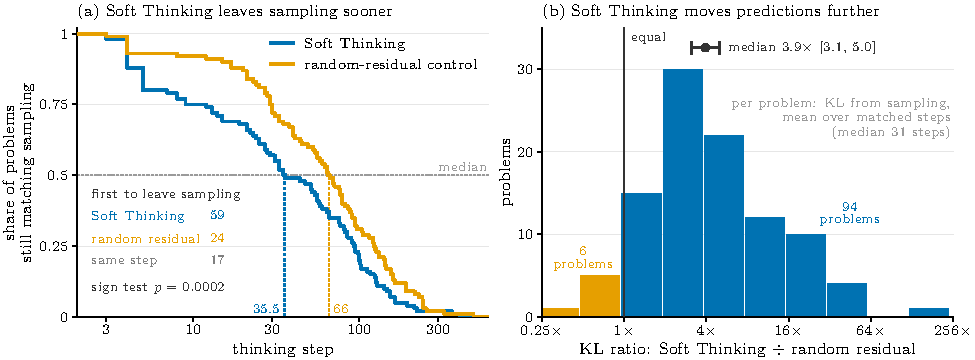
\includegraphics{fig7.pdf}
\caption{The model reads the residual.
Three arms run in lockstep with shared noise on 100 GSM8K problems: % C23.1
sampling (top token only), \ST{} (full blend) and a \ctrl{} (the residual moved to a random token).
(a) Share of problems on which each arm has so far picked the same token as sampling at every thinking step.
\ST{} leaves sampling sooner: median step 35.5 vs 66; % C23.4
it leaves first on 59 problems, the random residual on 24, both at once on 17 (sign test $p = 0.0002$). % C23.5-6
(b) Per problem, how far \ST{} moves next-token predictions away from sampling's, divided by how far the
random residual does (KL divergence, averaged over the steps before either arm leaves sampling;
median 31 steps). % C23.15
\ST{} moves them more on 94 of 100 problems; % C23.8
the median problem is 3.9 times (marker: median and 95\% bootstrap CI over problems, [3.1, 5.0]). % C23.15
Items 50--149, not used in any other experiment; seed 0.} % C23.1
\label{fig:ablation}
\end{figure}

\paragraph{The model reads the residual.}
\ST{} leaves sampling sooner than the \ctrl{} (\cref{fig:ablation}a).
The first step at which its token differs from sampling's has a median of 35.5, against 66 for the control. % C23.4
Paired by problem, \ST{} leaves first on 59 problems, the control on 24, and both at the same step on 17 % C23.5-6
(sign test, $p = 0.0002$). % C23.5-6
To compare the arms before their texts differ, we average the KL divergence of each arm's next-token
distribution from sampling's over the steps before either arm leaves sampling
(a median of 31 steps per problem). % C23.15
\ST{} moves the predictions more than the control on 94 of 100 problems. % C23.8
The median per-problem ratio is 3.9 (95\% CI [3.1, 5.0]; \cref{fig:ablation}b). % C23.15
We chose the median after seeing that the ratio of the means, 5.7, is driven by a few problems: % C23.14
five problems hold 0.54 of \ST{}'s total, and without them the ratio of means is 3.1. % C23.14
The pre-registered prediction E1 expected the opposite direction, that the residual would move predictions less than
a random one (\cref{app:prereg}).

\paragraph{Accuracy does not change detectably.}
\Cref{tab:accuracy} compares accuracy.
In Exp~23, \ST{} solves 88 of 100 problems and sampling 86. % C23.1
The discordant pairs split 6 to 4 (McNemar $p = 0.754$), % C23.2
and the two arms reach the same final answer on 84 problems. % C23.2
The \ctrl{} solves 82 (3 to 7 against sampling, $p = 0.344$), % C23.1 C23.3
and it also reaches sampling's final answer on 84 problems. % C23.3
So the real residual changes the final answer no more often than a random one.
In Exp~16, on different problems (items 0--29), \GST{} and sampling both solve 52 of 60 runs; % C16.1 C16.3
on seed 0, \GST{} alone is right on 1 problem and sampling alone on 2 ($p = 1.00$). % C16.12
Vanilla \ST{} shows the Greedy Pitfall of \citet{wu2025single} in its behaviour:
14 of its 30 runs end in Cold Stop, a repetition loop, % C16.2
and all of its 5 runs without an answer are among them. % C16.2 C16.8
\GST{} never hits Cold Stop, % C16.3
and sampling and \GST{} solve 4 of those 5 problems in every run. % C16.9
Vanilla's accuracy (22 of 30) is lower, but the difference is not significant at this size % C16.2
($p = 0.062$ against sampling, $p = 0.22$ against Gumbel). % C16.13 C16.5
These tests are small.
With only 6 and 4 discordant problems in Exp~23, an effect of a few points in either direction cannot be excluded. % C23.2
The pre-registered prediction E2 (no detectable accuracy difference, judged on the point estimate) was met.

\paragraph{Answer.}
The model reads the residual: it moves next-token predictions a median 3.9 times as much as a random residual of the % C23.15
same size, and it makes \ST{} leave sampling sooner.
Yet accuracy does not change detectably, and the real residual changes final answers no more often than a random one.
The residual is read but, within the power of our test, not used.
